\documentclass[../notes.tex]{subfiles}

\pagestyle{main}
\renewcommand{\chaptermark}[1]{\markboth{\chaptername\ \thechapter\ (#1)}{}}
\setcounter{chapter}{8}

\begin{document}




\chapter{Reaction Energetics}
\section{Equilibria}
\begin{itemize}
    \item \marginnote{10/29:}Lecture 14 continued: Examples of hydrogen bonds.
    \item Alex reviews strong, moderate, and weak hydrogen bonds (see Figure \ref{fig:intHbond} and discussion).
    \item Canonical hydrogen bonds.
    \begin{itemize}
        \item Those in the bifluoride anion (\ce{HF2-}).
        \begin{itemize}
            \item Held together by such a strong hydrogen bond that it is stable and isolable.
            \item Energy on the order of \kcal{39}.
        \end{itemize}
        \item Those between \ce{H2O} and \ce{H3O+}.
        \begin{itemize}
            \item Relatively strong, persistent in solution, etc.
            \item Energy on the order of \kcal{33}.
        \end{itemize}
        \item Those between \ce{H2O} and \ce{H2O}.
        \begin{itemize}
            \item The loss of the charge leads to a significant decrease in strength.
            \begin{itemize}
                \item Charge-assisted hydrogen bonds are typically stronger!
            \end{itemize}
            \item Energy on the order of \kcal{5}.
        \end{itemize}
        \item Fluoroform (\ce{CHF3}) in water.
        \begin{itemize}
            \item Energy on the order of \kcal{3}.
        \end{itemize}
    \end{itemize}
    \item Geometric parameters relevant to hydrogen bonding (find these in crystallographic/biological databases).
    \begin{itemize}
        \item Donor-acceptor bond length, and donor-acceptor bond angle.
    \end{itemize}
    \item The prevalence of different kinds of hydrogen bonds vs. the bond angle.
    \begin{figure}[H]
        \centering
        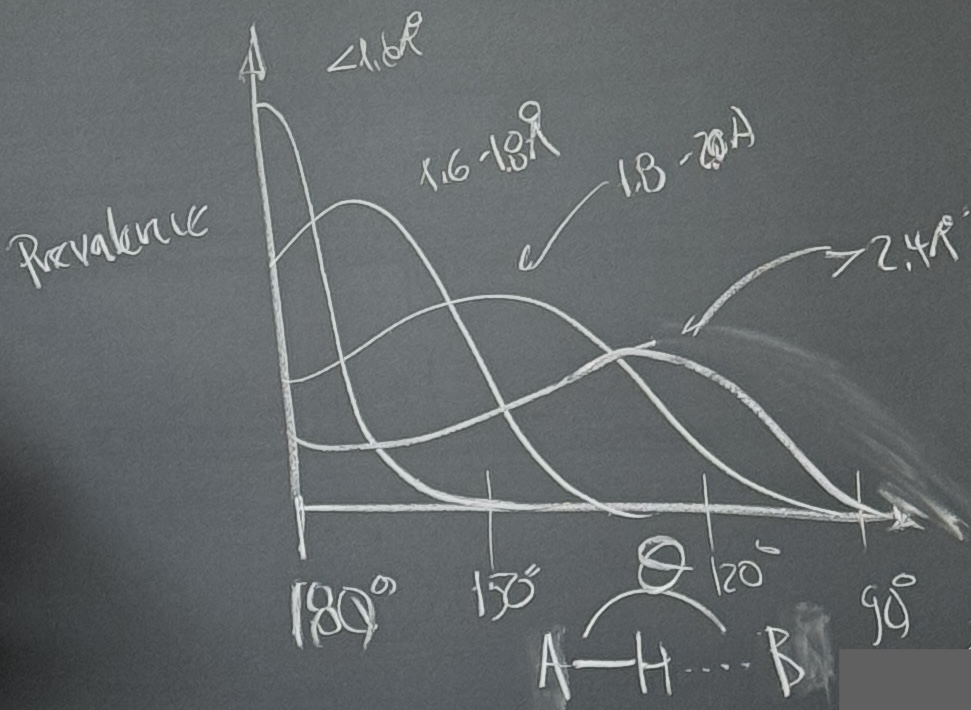
\includegraphics[width=0.4\linewidth]{HbondAng.JPG}
        \caption{Stronger hydrogen bonds are more linear.}
        \label{fig:HbondAng}
    \end{figure}
    \begin{itemize}
        \item We can think of this plot like a histogram.
        \item Takeaway: Stronger bonds are more linear, and weaker bonds are more bent.
        \item As the bond gets weaker, the molecules begin to explore a larger cone of orientations.
    \end{itemize}
    \item Example: \ce{H}-bonding in carbonyl species.
    \begin{figure}[h!]
        \centering
        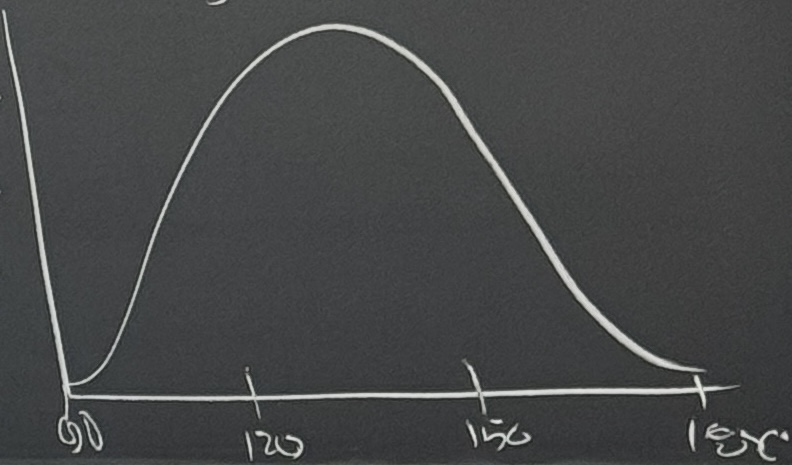
\includegraphics[width=0.4\linewidth]{HbondCarb.JPG}
        \caption{Carbonyl hydrogen bonds reflect \ce{O}($sp^2$) hybridization.}
        \label{fig:HbondCarb}
    \end{figure}
    \begin{itemize}
        \item We're looking at the carbonyl \ce{C=O^+-H} bond angle.
        \item These bonds cluster around an area consistent with protonation of one of the lone pairs.
        \item This indicates that protons' mobile electron density is held to static carbonyl electron density.
        \item What about thiocarbonyls? What if we replace oxygen with its heavier sulfur analog? This may be on PSet 3!!
    \end{itemize}
    \item Aside: \textcite{bib:Anslyn} replaced a much older, worse book.
    \begin{itemize}
        \item An ambitious book due to its breadth, but may alight or mangle details for a given topic.
        \item Suffice to say, it's the best book we've got.
    \end{itemize}
    \item \textbf{Hydrophobic effect}: It is energetically costly to solvate nonpolar molecules in \ce{H2O}.
    \begin{itemize}
        \item Dennis Dougherty's opinion: The hydrophobic effect is the most powerful force in biological chemistry.
    \end{itemize}
    \item Illustrating the hydrophobic effect.
    \begin{table}[h!]
        \centering
        \small
        \renewcommand{\arraystretch}{1.2}
        \begin{tabular}{cccc}
            \textbf{Solute} & \textbf{$\bm{\Delta G^\circ_\textbf{tr}}$ (kcal/mol)} & $\bm{\Delta H}$ & $\bm{-T\Delta S}$\\
            \hline
            \ce{PhH}             & $4.62$ & $0.50$ & $4.12$\\
            \ce{PhMe}            & $5.47$ & $0.41$ & $5.06$\\
            \emph{n}-\ce{hexane} & $7.78$ & $0.00$ & $7.78$\\
        \end{tabular}
        \caption{Hydrophobic effect examples.}
        \label{tab:hydrophobicEffect}
    \end{table}
    \begin{itemize}
        \item Defined by the energy penalty $\Delta G^\circ_\text{tr}$ to put a given solute in water.
        \item To put \emph{n}-hexane into water, it costs about $\Delta G^\circ_\text{tr}=\kcal{7.78}$.
        \begin{itemize}
            \item We can actually parse this in terms of its specific enthalpy and entropy.
            \item $\Delta H=0.00$. It's a wash in terms of dipole effects and energy interactions and everything.
            \item $-T\Delta S=7.78$. It's all in the entropy.
        \end{itemize}
        \item It's every so slightly more favorable to put benzene or toluene in water thermodynamically.
        \item Chemists are pretty good at estimating enthalpy, but pretty bad with entropy.
        \begin{itemize}
            \item Alex's goal for this class: We should all leave with a better understanding of entropy.
        \end{itemize}
        \item Conclusion: The energetic pentalty is mostly entropic.
        \begin{itemize}
            \item If we put a hydrophobic link in the water, it disrupts the water's ability to randomly hydrogen bond with itself.
            \item Less ability to \ce{H}-bond means less dynamic and more ordered water, driving the hydrophobic effect. This is the best hypothesis we have so far; it's still hard for Alex to wrap his head around.
            \item There's many chemists who study water, still!
        \end{itemize}
        \item References.
        \begin{itemize}
            \item \textcite{bib:HydrophobicEffect1}.
            \item \textcite{bib:HydrophobicEffect2}.
        \end{itemize}
    \end{itemize}
    \item We've indicated a couple of instances here where knowing a molecule's structure is not enough to predict it's reactivity!
    \begin{itemize}
        \item \emph{n}-hexane reacts differently as its own system vs. in \ce{H2O}.
        \item We need to appreciate with greater clarity how thermodynamics operate in chemical systems.
    \end{itemize}
    \item We now begin Lecture 15.
    \item Today: Reaction energetics.
    \begin{itemize}
        \item Goal for the next two lectures: Understand how differences in free energy impact\dots
        \begin{enumerate}[label={\arabic*)}]
            \item Equilibria (today);
            \item Kinetic rates (next time).
        \end{enumerate}
    \end{itemize}
    \item Overview concepts.
    \begin{itemize}
        \item Consider a reaction
        \begin{equation*}
            \ce{A <=> B}
        \end{equation*}
        \begin{itemize}
            \item How do we understand such a reaction on a systems level, rather than on a molecular basis?
        \end{itemize}
        \item A good place to start is with a reaction coordinate diagram.
        \begin{itemize}
            \item What we put on the $y$-axis will matter quite a bit.
            \begin{itemize}
                \item We'll stick with $\Delta E$ (generic energy change) for now, and then get to $\Delta G$.
            \end{itemize}
            \item The $x$-axis is the reaction coordinate along an arbitrarily defined interval 0-1.
            \item The minima relative heights of the energy minima for \ce{A} and \ce{B} give us information about the position $\Delta G_\text{rxn}$ of the equilibrium.
            \item This same formalism (with $\Delta G^\ddagger$) allows us to learn about the rate as well.
        \end{itemize}
    \end{itemize}
    \item Recall gas phase dissociation.
    \begin{figure}[H]
        \centering
        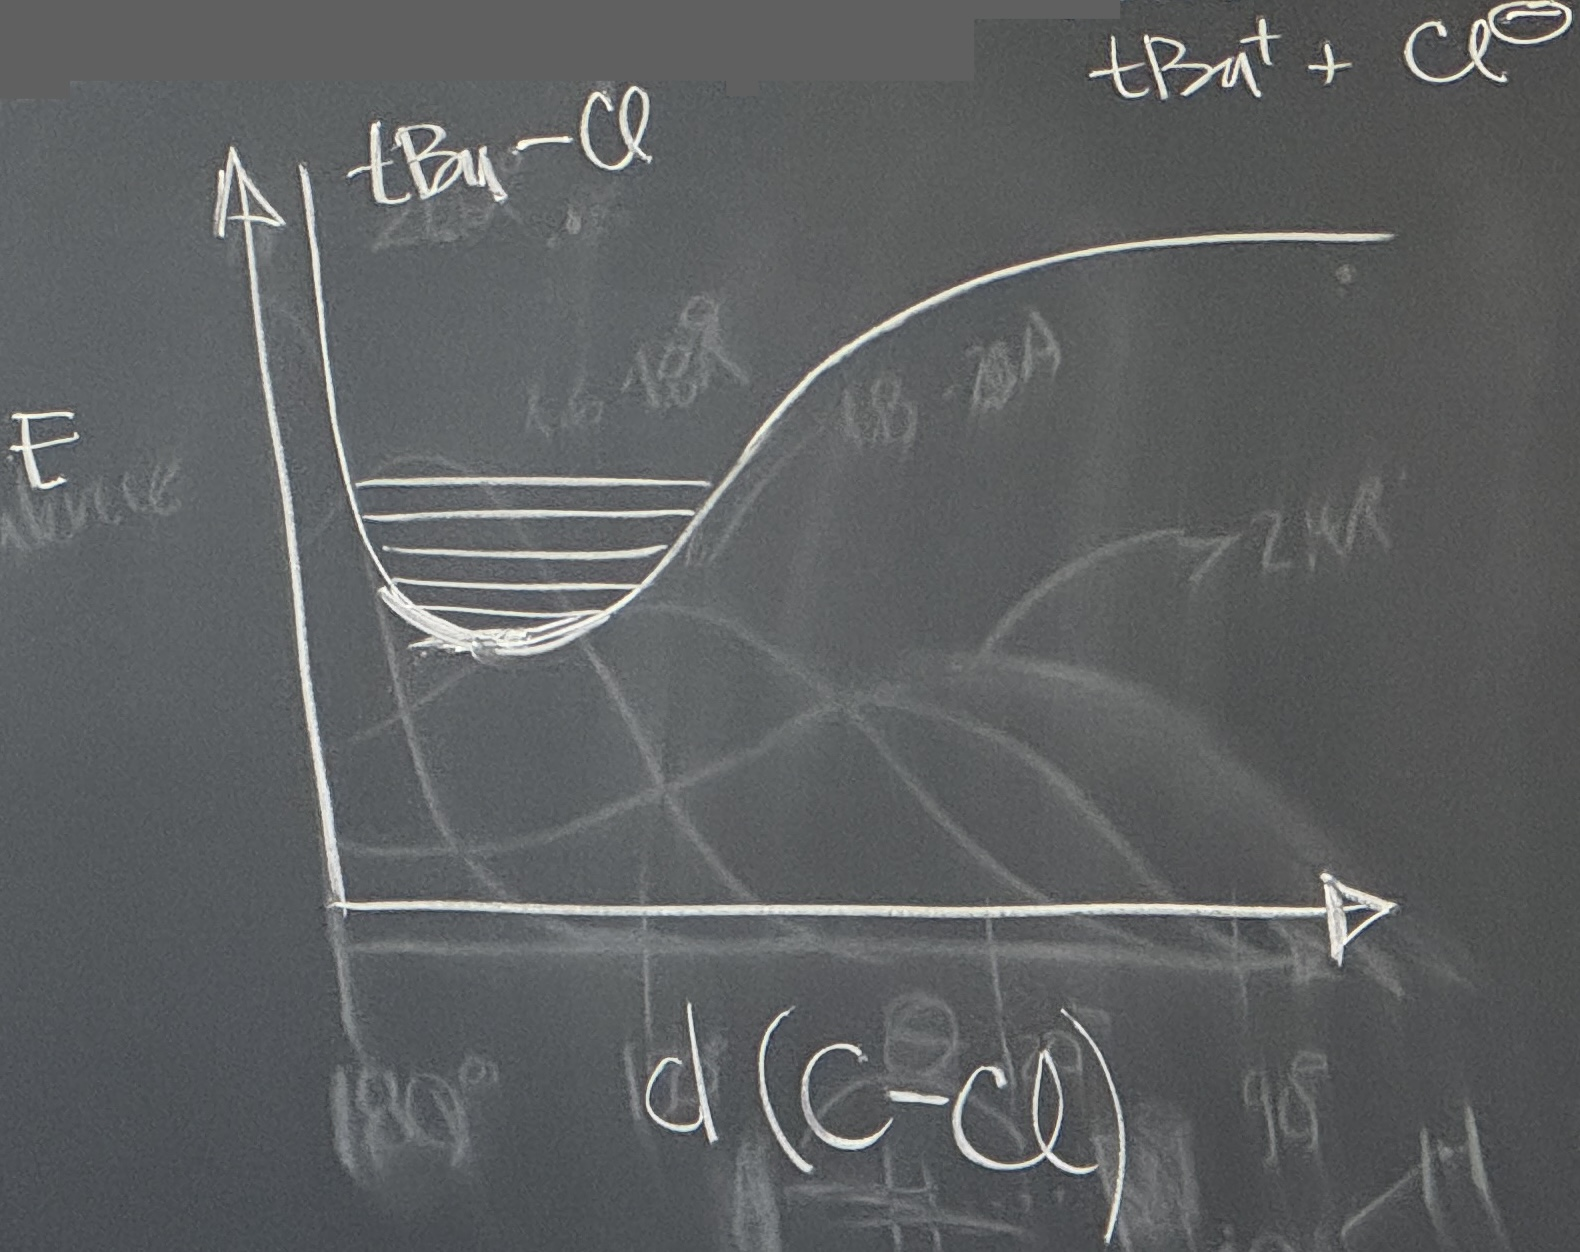
\includegraphics[width=0.4\linewidth]{EDtBuClgas.JPG}
        \caption{Energy diagram for the gas-phase dissociation of \emph{t}-butyl chloride.}
        \label{fig:EDtBuClgas}
    \end{figure}
    \begin{itemize}
        \item Consider \ce{{}^{\emph{t}}Bu-Cl}.
        \item The energy diagram is just Lennard-Jones, again.
        \item The vibrations of the \ce{C-Cl} bond along this potential surface are quantized. If you add enough energy, the ions can ping apart into \ce{{}^{\emph{t}}Bu+} and \ce{Cl-}.
        \item Most reactions do not occur in the gas phase, though; they occur in condensed media.
    \end{itemize}
    \item In the condensed phase, dissociation looks a bit different.
    \begin{figure}[h!]
        \centering
        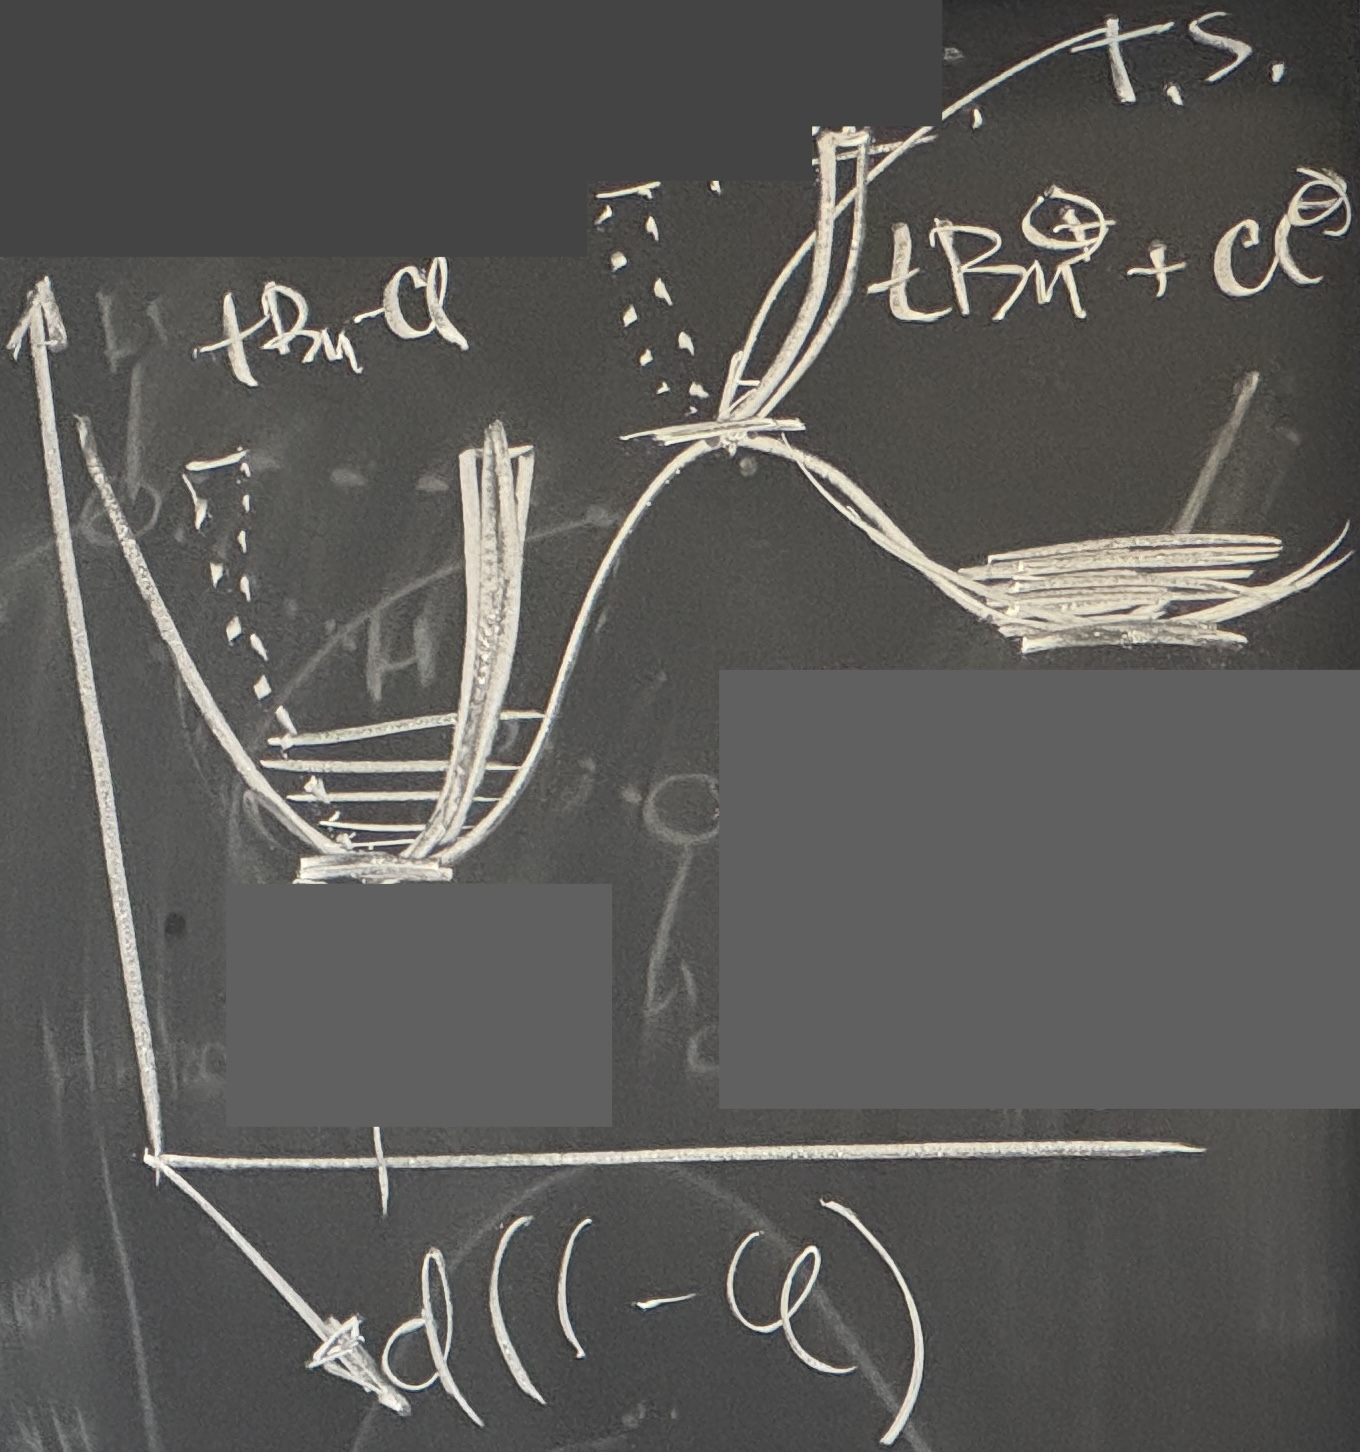
\includegraphics[width=0.3\linewidth]{EDtBuClcon.JPG}
        \caption{Energy diagram for the condensed-phase dissociation of \emph{t}-butyl chloride.}
        \label{fig:EDtBuClcon}
    \end{figure}
    \begin{itemize}
        \item Bonds are still stable, but the ions will now be stabilized by the condensed media.
        \item There is a transition state along the potential energy surface.
        \begin{itemize}
            \item This corresponds to some bond length where the atoms are separating but not yet solvated.
        \end{itemize}
        \item Degrees of freedom of a molecule: $3N-6$ or $3N-5$ degrees of vibrational freedom.
        \begin{itemize}
            \item Bear in mind that any potential energy surface that we draw is just a cut of the real surface.
            \item These graphs help by zooming in on a given reaction coordinate. We get to define this though; there's nothing intrinsic about one reaction coordinate over any other.
            \item Additional degrees of freedom may be represented as orthogonal paraboloids.
        \end{itemize}
        \item The total derivative of the multidimensional potential energy surface $\dv*{E}{r}=0$ at local minima.
        \item Let $r$ be the variable corresponding to our choice of reaction coordinate.
        \begin{itemize}
            \item $\pdv*[2]{E}{r}>0$ at stable structures along the reaction coordinate.
            \item $\pdv*[2]{E}{r}<0$ at the TS along the reaction coordinate.
        \end{itemize}
        \item TS's have to be \textbf{first-order saddle points}.
    \end{itemize}
    \item \textbf{First-order saddle point}: A point on a multidimensional surface that is a minimum along all the orthogonal vectors except one, on which it is maximized.
    \begin{itemize}
        \item In our case, the one vector along which the saddle point is maximized is the reaction coordinate.
    \end{itemize}
    \item Sergei: Why does the energy keep going up as the ions get farther apart? Shouldn't it just stop?
    \begin{itemize}
        \item The other well \emph{will} be anharmonically a well due to electrostatic interactions.
        \item It might keep going up very shallowly, but it will still keep going up.
        \item You can think of this as a residual effect of the solvated ions tugging on each other; even when solvated, opposite charges attract per the laws of physics, and it's more stable for them to be a meter apart than 2 meters apart.
    \end{itemize}
    \pagebreak
    \item We now look at two-state systems.
    \begin{itemize}
        \item This is a system in which two states \ce{A} and \ce{B} are in equilibrium via \ce{A <=>[K] B}.
        \item $K$ is defined by $K=[B]/[A]$.
        \item Energetically, $\Delta G=-RT\ln\Keq$ and hence $\Keq=\e[-\Delta G/RT]$.
    \end{itemize}
    \item Example: The two chair conformations of methylcyclohexane.
    \begin{itemize}
        \item At \SI{300}{\kelvin}, $\Keq=19/1$ in favor of the equatorial position.
        \item Here, $\Delta G=\kcal{1.74}$ (this is the A-value for a \ce{Me} group!).
    \end{itemize}
    \item We can generalize this to useful energies.
    \begin{table}[h!]
        \centering
        \small
        \renewcommand{\arraystretch}{1.2}
        \begin{tabular}{ccccc}
            \multicolumn{2}{c}{\underline{Species}} & \multicolumn{3}{c}{\underline{$\Delta G_\text{rxn}$ (kcal/mol)}}\\[1mm]
            $\bm{[\textbf{A}]}$ & $\bm{[\textbf{B}]}$ & $\bm{-78\,{}^\circ\textbf{C}=195\,\textbf{K}}$ & $\bm{\textbf{rt}=300\,\textbf{K}}$ & $\bm{100\,{}^\circ\textbf{C}=373\,\textbf{K}}$\\
            \hline
            1 & 1   & 0    & 0    & 0   \\
            1 & 2   & 0.27 & 0.41 & 0.51\\
            1 & 10  & 0.89 & 1.37 & 1.71\\
            1 & 100 & 1.78 & 2.74 & 3.41\\
        \end{tabular}
        \caption{Free energy differences required for a given product distribution at different temperatures.}
        \label{tab:energyProductTemp}
    \end{table}
    \begin{itemize}
        \item Different ratios of products have different $\Delta G_\text{rxn}$.
        \item The $\Delta G_\text{rxn}$ values are also different at different temperatures.
        \item Takeaways.
        \begin{itemize}
            \item The position of an equilibrium is temperature dependent.
            \item The energy differences needed to drive reactions significantly to completion are very small.
        \end{itemize}
        \item Bond enthalpies are huge; the chemistry that we do in the condensed phase is \emph{so} subtle.
        \begin{itemize}
            \item Designing new reactions requires mastering subtle energies.
        \end{itemize}
        \item The partition of species is given by Boltzmann distributions at different temperatures; this explains the table.
        \begin{itemize}
            \item Essentially, per the Maxwell-Boltzmann distribution, higher temperatures lead to increasing thermal populations of excited states, so it takes a bigger energy difference to maintain selectivity.
        \end{itemize}
    \end{itemize}
    \item A quantitative analysis of equilibria ($\Delta G^\circ$) is constituent of both\dots
    \begin{itemize}
        \item An enthalpy component ($\Delta H^\circ$);
        \begin{itemize}
            \item Units: \si[per-mode=symbol]{\kilo\calorie\per\mole}.
            \item Coming from bond strengths and NCIs.
            \item $\Delta H>0$ is endothermic; distinct from endergonic ($\Delta G>0$).
            \item $\Delta H<0$ is exothermic; distinct from exergonic ($\Delta G<0$).
        \end{itemize}
        \item An entropy component ($\Delta S^\circ$).
        \begin{itemize}
            \item Units: $\si{\entropyunit}=\si[per-mode=symbol]{\calorie\per\mole\per\kelvin}$.
            \item Entropy units are a measure of disorder.
            \item This is a reflection of Boltzmann's law on microstates, $S=R\ln\Omega$, where $\Omega$ is the number of microstates available.
        \end{itemize}
    \end{itemize}
    \pagebreak
    \item Experimental determination of $\Delta H^\circ$ and $\Delta S^\circ$: A \textbf{van't Hoff analysis}.
    \begin{itemize}
        \item Theoretically, begin finding a linear equation of the form $y=mx+b$ where $m$ and $b$ correspond to $\Delta H^\circ$ and $\Delta S^\circ$, and $y$ and $x$ correspond to observables. In particular, we find
        \begin{align*}
            -RT\ln\Keq &= \Delta H^\circ-T\Delta S^\circ\\
            R\ln\Keq &= -\Delta H^\circ\left( \frac{1}{T} \right)+\Delta S^\circ
        \end{align*}
        \begin{itemize}
            \item Note that the first equality comes from the fact that the quantities on both sides of the equation equal $\Delta G^\circ$.
        \end{itemize}
        \item So we experimentally measure $\Keq$ at a range of temperatures and then use linearization to determine $\Delta H^\circ$ and $\Delta S^\circ$.
        \item These are super fun and satisfying to do because when it works, you can just read out the chemical potential directly from an observable.
        \item Massive caveat: There are a limited range of temperatures under which an equilibrium can be established.
        \begin{itemize}
            \item So we're only assaying an extremely small temperature range.
            \item Thus, small systematic errors can lead to wide variation in the extrapolated values. So we need to treat these analyses with care.
        \end{itemize}
    \end{itemize}
    \item Moving on, consider a bimolecular reaction.
    \begin{itemize}
        \item For example, consider oxidative addition of an aryl chloride to a palladium catalyst.
        \begin{itemize}
            \item Two things become one in this step.
        \end{itemize}
        \item The reaction enthalpy will obviously depend on the bonds broken and formed, but what will be the qualitative sense of entropy?
    \end{itemize}
    \item Qualitative prediction of equilibria.
    \begin{itemize}
        \item How do we estimate the position?
        \item Proton-transfer values can be helpful.
        \begin{itemize}
            \item \ce{AH + B -> A- + HB+}.
            \item Proton affinity and acidity report indirectly on the stability of the conjugate bases.
            \item $\pKa=-\log\Ka$, so $\Delta G=-1.4\pKa$. "A log unit gives \kcal{1.4}." Therefore, we can know something about the energetics by looking at this reactive intermediate!
        \end{itemize}
        \item We can also follow \ce{H}-atom transfers.
        \begin{itemize}
            \item Look at alkane transfers; $\Delta\text{BDE}=\Delta H$.
            \item Hydride ion affinity can also help us; these values are tabulated with respect to cation stability.
        \end{itemize}
        \item How do we estimate the entropy?
        \begin{itemize}
            \item A fragmention releases about \eu{30}, and a joining of a catalyst to a molecule costs about \eu{30}. \eu{30} times \SI{300}{\kelvin} gives you about \kcal{9}! So the new bonds formed must exceed \kcal{9}.
            \item You can't just do bonds formed and broken; "nah, man; you need \kcal{9}; that's real energy!"
        \end{itemize}
    \end{itemize}
\end{itemize}
\newpage



\section{Transition State Theory}
\begin{itemize}
    \item \marginnote{10/31:}Lecture 15 continued.
    \item Consider a simple equilibria of the following form.
    \begin{equation*}
        \ce{A <=> B}
    \end{equation*}
    \begin{itemize}
        \item We can characterize it by $\Delta G=-RT\ln\Keq$.
        \item We can parse $\Delta G$ in terms of $\Delta H$ and $\Delta S$ using the van't Hoff analysis.
        \item We now show that $\ln\Keq$ (and hence $\Keq$) is unitless for this equilibrium.
        \begin{itemize}
            \item Units of $\Delta G$: \si[per-mode=symbol]{\kilo\calorie\per\mole}.
            \item Units of $T$: Temperature.
            \item Units of $R$: \si[per-mode=symbol]{\kilo\calorie\per\mole\per\kelvin}.
            \item Therefore, $\ln\Keq$ is unitless since all units cancel in the equivalent fraction $\Delta G/RT$.
            \item It follows that $\Keq$ is unitless.
            \item We can also see this from the fact that the two molarity units cancel.
        \end{itemize}
        \item We can also characterize the equilibrium constant as $\Keq=\cnc{B}/\cnc{A}$.
    \end{itemize}
    \item We can have much more complex equilibria, too, such as multicomponent equilibria.
    \item Consider the following associative equilibrium.
    \begin{equation*}
        \ce{A + B <=> C}
    \end{equation*}
    \begin{itemize}
        \item Here,
        \begin{equation*}
            \Keq = \frac{\cnc{C}}{\cnc{A}\cnc{B}}
        \end{equation*}
        \item Hence, $\Keq$ has units of \si{\per\molar}.
        \item This implies that $\Delta G$ is concentration dependent!
        \begin{itemize}
            \item This is a profound statement.
        \end{itemize}
    \end{itemize}
    \item Consequence: A catalyst operating on a starting material.
    \begin{equation*}
        \ce{cat + SM <=>[$\Keq$] cat*SM -> P}
    \end{equation*}
    \begin{itemize}
        \item Example: TM catalyst on organic substrate, enzyme on a biological substrate.
        \item Assume: $\Keq=100$ and 1 mol\% catalyst.
        \item Let's think about this reaction sequence.
        \begin{itemize}
            \item Consider the percent of catalyst bound by the starting material, i.e.,
            \begin{equation*}
                \frac{\cnc{cat*SM}}{\cnc[T]{cat}}
            \end{equation*}
            where $\cnc[T]{cat}$ is the \underline{t}otal amount of catalyst, bound and unbound.
            \item During the course of the reaction, the position of the equilibrium will decay. At some point, there will be more catalyst than SM!
            \item Case A (near \SI{1}{\molar} SM): On a potential energy surface, \ce{cat*SM} (the catalyst resting state) is lower in energy than the complex.
            \item Case B (low SM concentration): Less \ce{cat*SM} at equilibrium. So potential energy surfaces are \emph{not} static; they can depend on concentrations.
            \item It's not $\Keq$ changing, but that $Q$ is concentration dependent?? But $Q$ can change $\Delta G$, sure.
        \end{itemize}
    \end{itemize}
    \item So how do we standardize conditions to standard states?
    \begin{itemize}
        \item Use $\Delta G^\circ$, $\Delta H^\circ$, and $\Delta S^\circ$!
    \end{itemize}
    \item Defining a standard state.
    \begin{equation*}
        \ce{A <=> B}
    \end{equation*}
    \begin{itemize}
        \item Consider a simple two-state equilibrium to start, like the above.
        \item Define the equilibrium constant $\Keq$ as before.
        \begin{equation*}
            \Keq = \frac{\cnc[eq]{B}}{\cnc[eq]{A}}
        \end{equation*}
        \item We now define another ratio at some arbitrary time $t$ with some non-equilibrium concentrations.
        \begin{equation*}
            Q = \frac{\cnc[$t$]{B}}{\cnc[$t$]{A}}
        \end{equation*}
        \item Then we can define the free energy $\Delta G$ of a system at any time point with respect to the equilibrium!
        \begin{equation*}
            \Delta G = -RT\ln(\frac{\Keq}{Q})
            = \Delta G^\circ+RT\ln Q
        \end{equation*}
        \begin{itemize}
            \item This value tells us the tendency of the reaction to proceed to equilibrium under \emph{any} conditions.
            \item You can also think of this as the driving force at a given time point.
            \item This \emph{rigorously} tells us that $\Delta G=0$ at equilibrium.
        \end{itemize}
        \item We can also define the standard state
        \begin{equation*}
            \Delta G^\circ = -RT\ln\Keq
        \end{equation*}
        in which $Q=1$.
        \begin{itemize}
            \item This value tells us about the tendency of the reaction to proceed to equilibrium under \emph{standard} conditions.
        \end{itemize}
    \end{itemize}
    \item Example: Assume $\Keq=3$ in a simple equilibrium \ce{A <=> B}.
    \begin{figure}[h!]
        \centering
        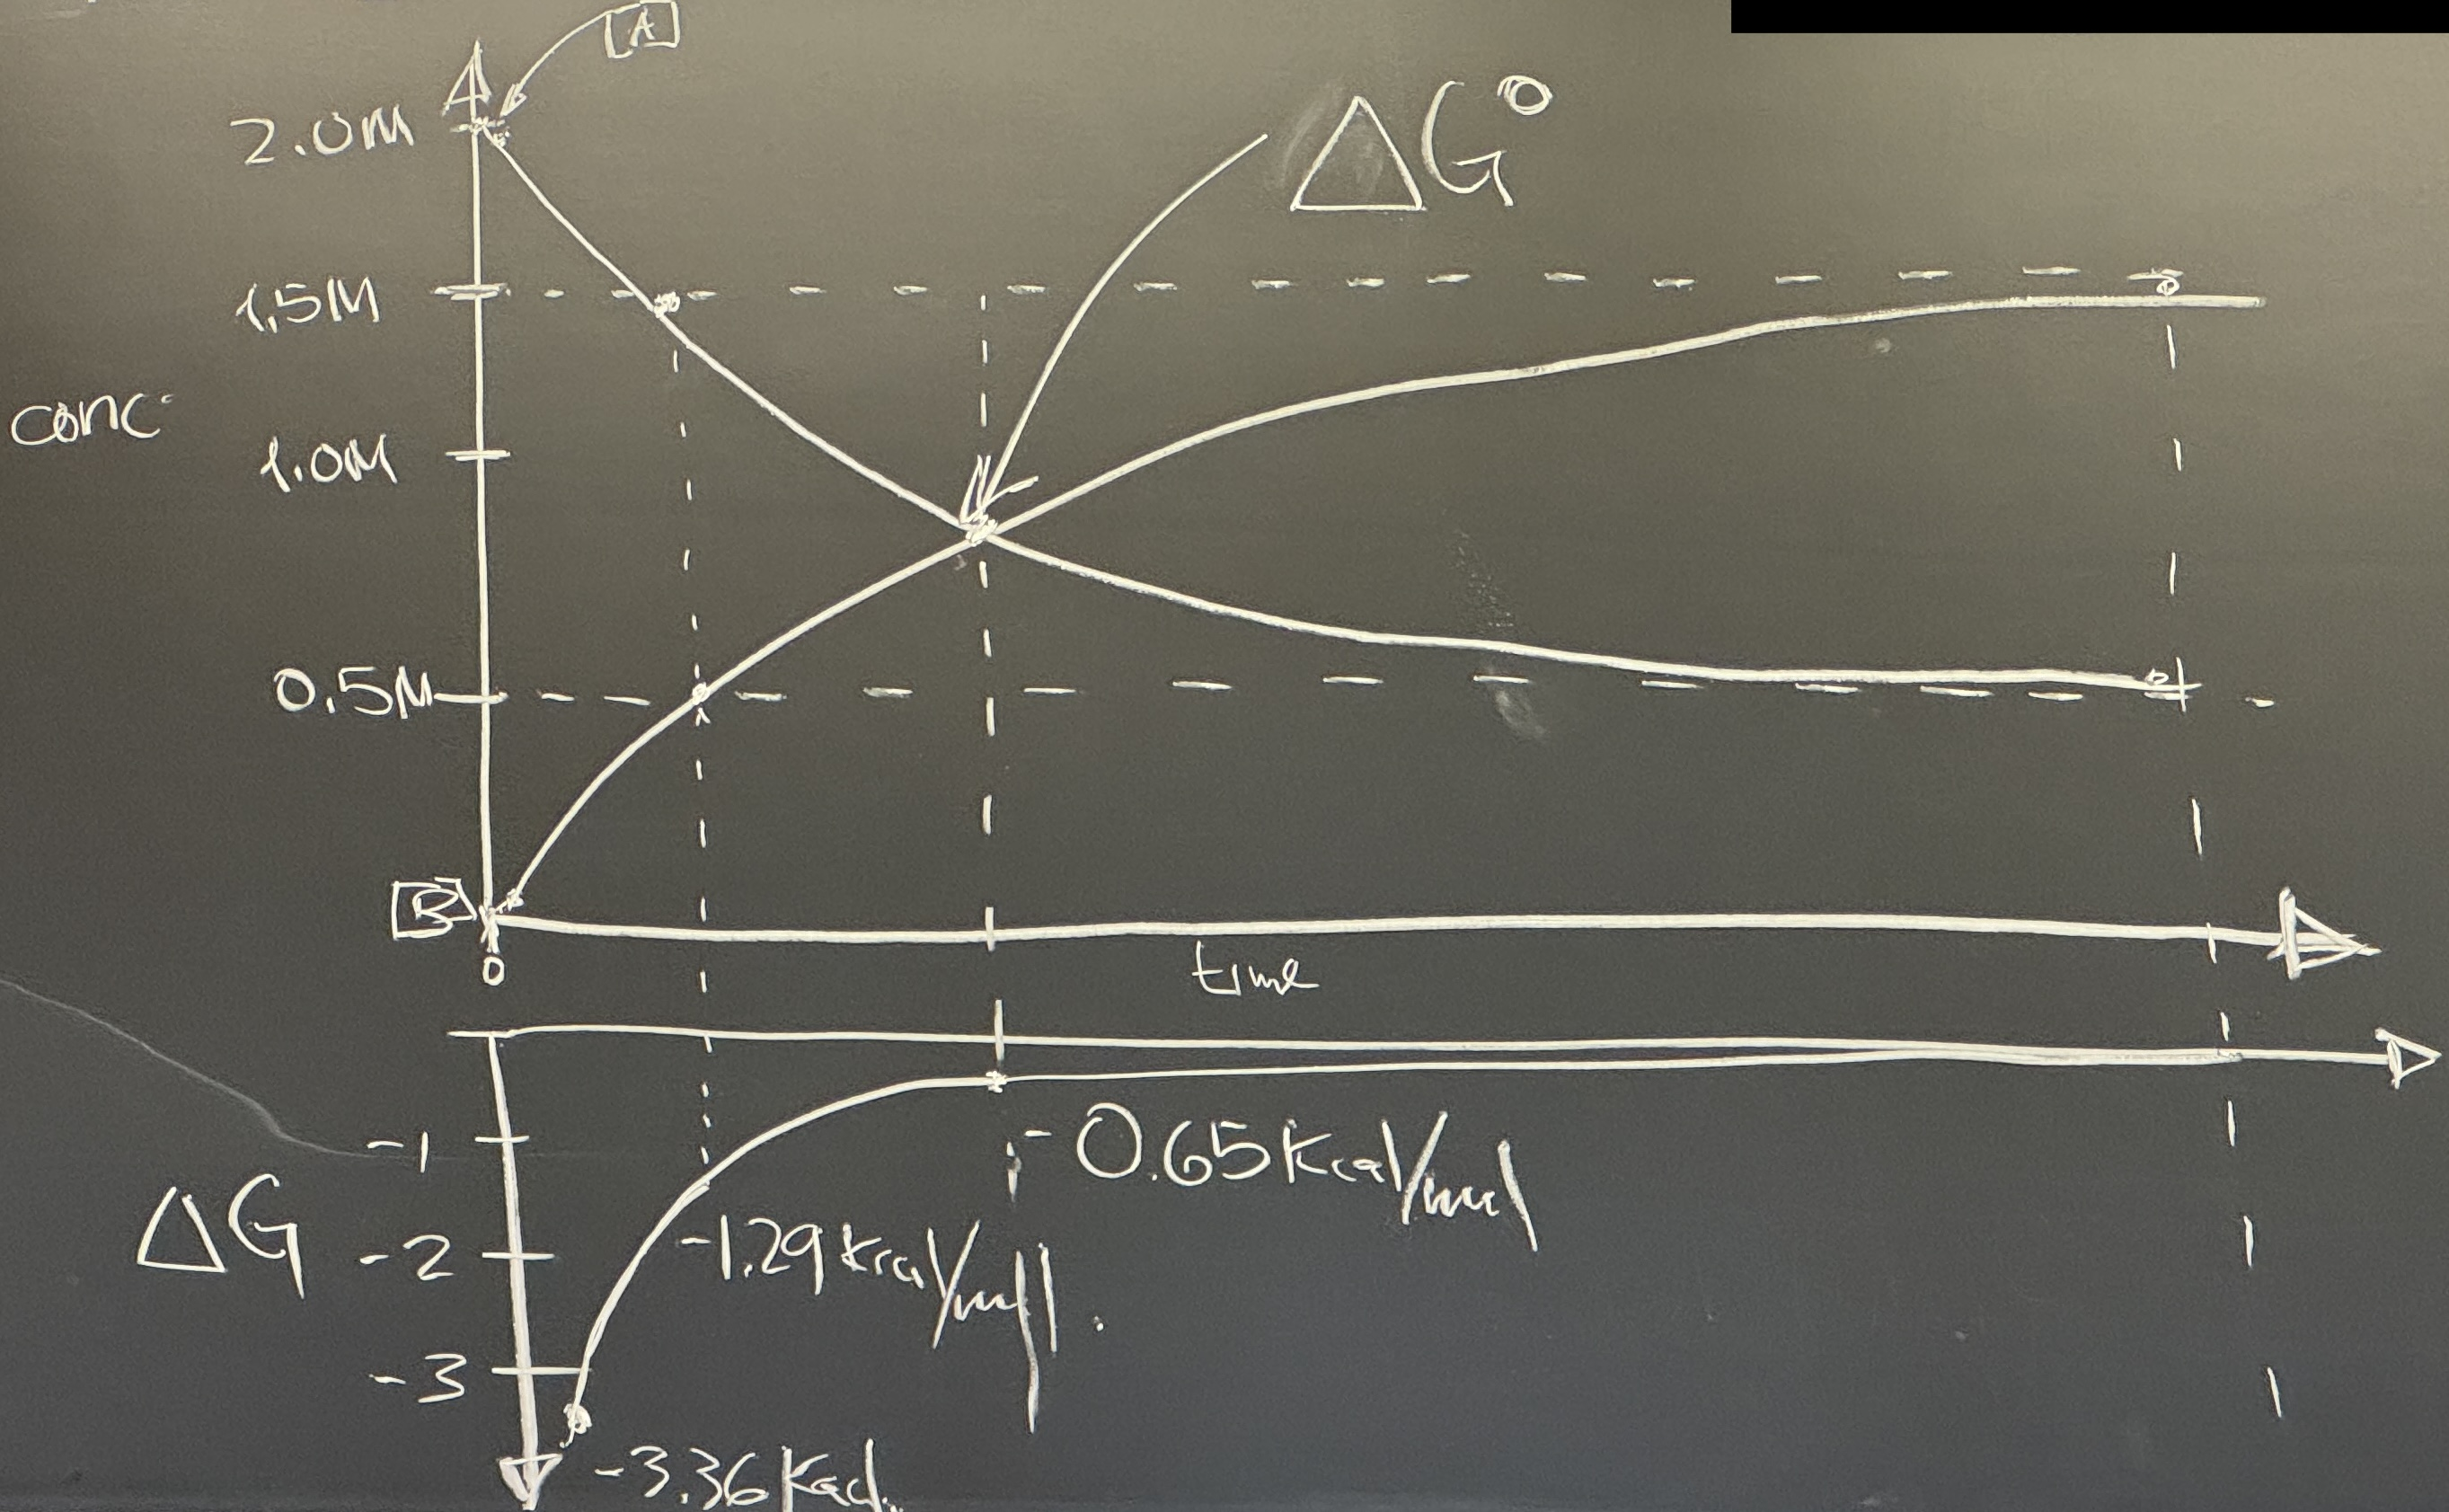
\includegraphics[width=0.65\linewidth]{timeCourseNrg.JPG}
        \caption{A time course vs. free energy.}
        \label{fig:timeCourseNrg}
    \end{figure}
    \pagebreak
    \begin{itemize}
        \item Let $\cnc[0]{A}=\SI{2}{\molar}$ and $\cnc[0]{B}=\SI{0}{\molar}$.
        \item Then in the end, $\cnc[eq]{A}=\SI{0.5}{\molar}$ and $\cnc[eq]{B}=\SI{1.5}{\molar}$.
        \item Consider a time course, i.e., how the concentrations change in time.
        \item After mixing the compounds, as quickly as we can get to the NMR, we take a time point.
        \begin{itemize}
            \item So $\cnc[1]{A}<\SI{2}{\molar}$ and $\cnc[1]{B}>\SI{0}{\molar}$ slightly.
            \item Suppose that specifically, $\cnc[1]{A}=\SI{1.98}{\molar}$ and $\cnc[1]{B}=\SI{0.02}{\molar}$.
            \item Then $Q_1=0.01$, so $\Delta G_1=-\kcal{3.36}$.
        \end{itemize}
        \item Now underneath, we plot the free energy vs. time.
        \item $\cnc{A}$ decreases to equilibrium and $\cnc{B}$ increases to equilibrium over time.
        \item Second time point.
        \begin{itemize}
            \item Suppose that specifically, $\cnc[2]{A}=\SI{1.5}{\molar}$ and $\cnc[2]{B}=\SI{0.5}{\molar}$.
            \item Then $Q_2=0.33$, so $\Delta G_2=-\kcal{1.29}$.
        \end{itemize}
        \item Third time point.
        \begin{itemize}
            \item Suppose that specifically, $\cnc[3]{A}=\SI{1}{\molar}$ and $\cnc[3]{B}=\SI{1}{\molar}$.
            \item Then $Q_3=1$, so $\Delta G_3=-\kcal{0.65}$.
        \end{itemize}
        \item Fourth time point.
        \begin{itemize}
            \item Suppose that specifically, $\cnc[$\infty$]{A}=\SI{0.5}{\molar}$ and $\cnc[$\infty$]{B}=\SI{1.5}{\molar}$.
            \item Then $Q_\infty=3$, so $\Delta G_\infty=\kcal{0}$.
        \end{itemize}
        \item The third time point is $\Delta G^\circ$ since $Q=1$!
        \begin{itemize}
            \item So standard conditions start to tell us a bit about how the reaction goes.
        \end{itemize}
    \end{itemize}
    \item This concludes Lecture 15.
    \item Today: Transition state theory.
    \item Empirical observation: The rate of the reaction is proportional to the following.
    \begin{equation*}
        \text{rate} = A\e[-E_a/RT]
    \end{equation*}
    \begin{itemize}
        \item This is the \textbf{Arrhenius law}.
        \item Even before we knew what atoms were, we could track the process of a reaction.
        \item What unified and predicted the Arrhenius law was a theoretical development from the 1930s called Transition State Theory.
    \end{itemize}
    \item Two key assumptions.
    \begin{enumerate}
        \item A so-called "activated complex" may be viewed as being in quasi-equilibrium with the starting material.
        \begin{itemize}
            \item Essentially, reformulate \ce{A -> B} as
            \begin{equation*}
                \ce{A <=>[$K^\ddagger$] [TS] ->[$k^\ddagger$] B}
            \end{equation*}
            \item This allows us to bring to bear our mathmatical treatment of equilibria on a kinetic argument.
            \item Call the quasi-equilibrium constant $K^\ddagger$, where
            \begin{equation*}
                K^\ddagger = \frac{\cnc{TS}}{\cnc{A}}
            \end{equation*}
        \end{itemize}
        \item Any molecule that makes its way to the transition state will then proceed onto the product barrierlessly.
    \end{enumerate}
    \item Thus, we can say that the rate of reaction is given by the following.
    \begin{equation*}
        \text{rate} = \dv{\cnc{B}}{t}
        = k^\ddagger\cnc{TS}
        = K^\ddagger k^\ddagger\cnc{A}
    \end{equation*}
    \begin{itemize}
        \item This winds up being useful for a variety of reasons.
        \item In particular, we can extrapolate this simple analysis to other processes with higher molecularity.
    \end{itemize}
    \item Example: We can learn the stoichiometry of the rate law just by analysis of the reaction equation. Consider
    \begin{equation*}
        \ce{$a$A + $b$B + $c$C -> D}
    \end{equation*}
    \begin{itemize}
        \item Then
        \begin{align*}
            K^\ddagger &= \frac{\cnc{TS}}{\cnc{A}^a\cnc{B}^b\cnc{C}^c}\\
            \cnc{TS} &= K^\ddagger\cnc{A}^a\cnc{B}^b\cnc{C}^c
        \end{align*}
        \item This means that
        \begin{equation*}
            \text{rate} = K^\ddagger k^\ddagger\cnc{A}^a\cnc{B}^b\cnc{C}^c
        \end{equation*}
        \begin{itemize}
            \item So we can learn about the components of the transition structure just by inspecting the rate law.
        \end{itemize}
    \end{itemize}
    \item Example: Multistep sequences.
    \begin{equation*}
        \ce{\tfrac{1}{2}cat*cat + A <=> cat + A -> B}
    \end{equation*}
    \begin{itemize}
        \item Imagine if the catalyst can either bind to \ce{A} or off-cycle by dimerizing.
        \item This tells us something about the potential energy surface.
        \begin{itemize}
            \item The overall rate-determining energy span covers not just the forward direction, but the off-cycling!
        \end{itemize}
        \item This means that the catalyst has fractional order in the rate law.
        \begin{equation*}
            \text{rate} = k\cnc{A}\cnc{cat}^{1/2}
        \end{equation*}
        \begin{itemize}
            \item Note that $k=K^\ddagger k^\ddagger$.
            \item This tells us something about the transition state structure relative to the ground state, so knowing what the ground state is is essential.
        \end{itemize}
        \item If we have a minor equilibrium on the other hand, then
        \begin{equation*}
            \text{rate} = k\cnc{A}\cnc{cat}
        \end{equation*}
    \end{itemize}
    \item Note that the transition state structure has a lifetime on the order of bond vibrations.
    \item Sergei: All the k's?
    \begin{itemize}
        \item $K$: Equilibrium constant.
        \item $K^\ddagger$: Equilibrium constant to the transition structure.
        \item $k$: Experimental or apparent rate constant.
        \item $k^\ddagger$: Kinetic efficiency of the transition structure proceeding to product.
        \item $\kappa$: We'll get there.
        \item $\kB$: The Boltzmann constant.
    \end{itemize}
    \pagebreak
    \item Recall \ce{{}^{\emph{t}}BuCl -> {}^{\emph{t}}Bu+ + Cl-}.
    \begin{itemize}
        \item The rate for the formation of the product is given as
        \begin{equation*}
            \text{rate} = \dv{\cnc{B}}{t} = K^\ddagger k^\ddagger\cnc{A}
        \end{equation*}
        \item The facility with which the reaction proceeds is mostly \ce{C-Cl} bond cleavage, so $k^\ddagger$ must largely be proportional to a fudge factor $\kappa$ (the transmission coefficient) times $\nu$ (the frequency associated with the relevant bond).
        \begin{equation*}
            k^\ddagger = \kappa\nu
        \end{equation*}
        \begin{itemize}
            \item In reality, this frequency will be the "imaginary frequency" at the transition state, not any real-numbered frequency.
        \end{itemize}
        \item The point: There is a derivation in statistical mechanics through which we can more formally think about this.
        \begin{itemize}
            \item We get
            \begin{equation*}
                K^\ddagger = \left( \frac{\kB T}{h\nu} \right)\e[-\Delta G^\ddagger/RT]
            \end{equation*}
            \begin{itemize}
                \item $h$ is Planck's constant.
            \end{itemize}
            \item Then we bring this together with the above to get
            \begin{equation*}
                \text{rate} = \dv{\cnc{B}}{t} = \left[ \kappa\left( \frac{\kB T}{h} \right)\e[-\Delta G^\ddagger/RT] \right]\cnc{A}
            \end{equation*}
            \item From here, we can get the \textbf{Eyring equation}:\footnote{See CHEM26300Notes for the derivation.}
            \begin{equation*}
                k = K\left( \frac{\kB T}{h} \right)\e[-\Delta G^\ddagger/RT]
            \end{equation*}
        \end{itemize}
    \end{itemize}
    \item David: Does the Eyring equation condense into the Arrhenius equation?
    \begin{itemize}
        \item Short answer: No, but they're close.
        \item Devil's in the details: It depends on what exactly is meant by "activation energy." Additionally, in real life, the activated complex \emph{can} rebound back into the starting material.
    \end{itemize}
    \item The Eyring analysis allows us to predict a rate constant from an energy barrier, and vice versa.
    \item A few useful points.
    \begin{table}[h!]
        \centering
        \small
        \renewcommand{\arraystretch}{1.2}
        \begin{tabular}{ccc}
            \textbf{$\bm{\Delta G^\ddagger}$ (kcal/mol)} & \textbf{$\bm{k}$ ($\bm{\textbf{s}^{-1}}$)} & \textbf{$\bm{\tau_{1/2}}$ (s)}\\
            \hline
            \num{3}  & \num{3.8e10}  & \num{1.8e-11}\\
            \num{10} & \num{2.7e5}   & \num{2.5e-6}\\
            \num{15} & \num{5.9e1}   & \num{1.2e-2}\\
            \num{20} & \num{1.3e-2}  & \num{55}\\
            \num{25} & \num{2.7e-6}  & \SI{70}{\hour}\\
            \num{30} & \num{5.8e-10} & \SI{38}{\year}\\
        \end{tabular}
        \caption{Relating the energy barrier to the rate.}
        \label{tab:energyRate}
    \end{table}
    \begin{itemize}
        \item Let's define $\Delta G^\ddagger$ (in \si[per-mode=symbol]{\kilo\calorie\per\mole} at \SI{298}{\kelvin}), the rate constant $k$ (in \si{\per\second}), and the half-life $\tau_{1/2}$ (in \si{\second}).
        \item Example of a \kcal{3} process: Ethane bond rotation.
    \end{itemize}
    \item Begin to internalize common kcal values!!
    \begin{itemize}
        \item Print out a list and put it next to tooth-brushing mirror.
    \end{itemize}
\end{itemize}




\end{document}